\documentclass[12pt, a4paper]{article}
\usepackage[a4paper,top=1.5cm, bottom=1.5cm, left=2cm, right=2cm]{geometry}
\usepackage{graphicx} % Required for inserting images
%%% Работа с русским языком
\usepackage{cmap}					% поиск в PDF
\usepackage{mathtext} 				% русские буквы в фомулах
\usepackage[T2A]{fontenc}			% кодировка
\usepackage[utf8]{inputenc}			% кодировка исходного текста
\usepackage[english,russian]{babel}	% локализация и переносы
\usepackage{float}
\usepackage{subcaption}
\usepackage{wrapfig}
\usepackage{tabularx}
\usepackage{multirow}

\usepackage[unicode, colorlinks=true, urlcolor=blue]{hyperref}
\usepackage[rgb]{xcolor}
\hypersetup{
colorlinks=true,urlcolor=blue
}
%%% Дополнительная работа с математикой
\usepackage{amsmath,amsfonts,amssymb,amsthm,mathtools} % AMS
\usepackage{icomma} % "Умная" запятая: $0,2$ --- число, $0, 2$ --- перечисление
%% Номера формул
\mathtoolsset{showonlyrefs=true} % Показывать номера только у тех формул, на которые есть \eqref{} в тексте.
%% Шрифты
\usepackage{euscript}	 % Шрифт Евклид
\usepackage{mathrsfs} % Красивый матшрифт
%% Свои команды
\DeclareMathOperator{\sgn}{\mathop{sgn}}
%% Перенос знаков в формулах (по Львовскому)
\newcommand*{\hm}[1]{#1\nobreak\discretionary{}
{\hbox{$\mathsurround=0pt #1$}}{}}


\usepackage{indentfirst}
% \usepackage[italicdiff]{physics}
\graphicspath{{images/}}
\DeclareGraphicsExtensions{.pdf,.png,.jpg}
\usepackage{enumitem}
\usepackage{caption}
\usepackage{array}
\usepackage{ragged2e}

\usepackage{tikz}
\usetikzlibrary{arrows,decorations.markings,calc}
\usetikzlibrary{arrows.meta, calc, patterns}







\begin{document}



\include{titlepage}
\begin{titlepage}
\thispagestyle{empty}

\begin{center}
\small
Министерство науки и высшего образования Российской Федерации\\[2mm]
\textbf{ФЕДЕРАЛЬНОЕ ГОСУДАРСТВЕННОЕ АВТОНОМНОЕ
ОБРАЗОВАТЕЛЬНОЕ УЧРЕЖДЕНИЕ ВЫСШЕГО ОБРАЗОВАНИЯ}\\[1mm]
«МОСКОВСКИЙ ФИЗИКО-ТЕХНИЧЕСКИЙ ИНСТИТУТ\\
(НАЦИОНАЛЬНЫЙ ИССЛЕДОВАТЕЛЬСКИЙ УНИВЕРСИТЕТ)»\\
(МФТИ, Физтех)
\end{center}

\vspace{18mm}

\begin{center}
\large \textbf{КАФЕДРА КВАНТОВОЙ ЭЛЕКТРОНИКИ}\\[10mm]
\Large \textbf{ОТЧЁТ}\\[2mm]
\large \textbf{ПО ЛАБОРАТОРНОЙ РАБОТЕ}\\[14mm]
\Large \textbf{Использование твердотельного YAG:Nd$^{3+}$-лазера с модуляцией добротности для гравировки материалов}
\end{center}

\vfill

% Блоки с подписями слева, линии и пояснения справа
\noindent
\begin{tabular}{@{}p{0.44\linewidth}p{0.52\linewidth}@{}}
\textit{Работу выполнили:} & Вакорина Анастасия,

Винокуров Владислав,

Выгнанчук Валерия,

Ескина Ольга,

Рагозина Елизавета,

Струков Олег,

Группа Б04-404 \\[8mm]

\textit{Работу принял, оценка:} & \\[3mm]
 \\
\end{tabular}


\vspace{12mm}

\begin{center}
\small Долгопрудный, \the\year{}~г.
\end{center}

\end{titlepage}








\newpage





\section*{Теоретическая часть}

\subsection*{Физические основы процесса лазерной гравировки}
В основе лазерной гравировки и маркировки материалов лежит тепловое воздействие излучения на вещество. В процессе обработки происходит нагревание, плавление и испарение части материала с образованием углублений, формирующих рельефное изображение. Энергия, затрачиваемая на нагрев ($Q_1$), плавление ($Q_2$) и испарение ($Q_3$), описывается классическими соотношениями:
\begin{equation}
    Q_1 = c m \Delta t, \quad Q_2 = \lambda m, \quad Q_3 = L m,
\end{equation}
где $m$ --- масса материала, $c$ --- удельная теплоемкость, $\Delta t$ --- изменение температуры, $\lambda$ и $L$ --- удельные теплоты плавления и парообразования соответственно.

Лазерное излучение, падая на поверхность, частично отражается, а частично проникает вглубь материала. Изменение плотности потока излучения описывается законом Бугера--Ламберта:
\begin{equation}
    I(x) = I_0 A \exp\left(-\int_0^x \alpha(x') dx'\right),
\end{equation}
где $I_0$ --- интенсивность падающего излучения, $A = 1 - R$ --- коэффициент поглощения ($R$ --- коэффициент отражения), $\alpha$ --- линейный коэффициент поглощения. Для большинства металлов коэффициент отражения увеличивается с ростом длины волны падающего излучения (например, для алюминия при $\lambda = 1{,}064$ мкм $R \approx 0{,}93$).

Дальнейшее распределение тепла в материале определяется уравнением теплопроводности:
\begin{equation}
    \frac{\partial T}{\partial t} - a \nabla^2 T = \frac{\alpha(x) q(y,z,t) \exp\left(-\int_0^x \alpha(x') dx'\right)}{\rho C},
\end{equation}
где $a$ --- температуропроводность, $\rho C$ --- удельная объемная теплоемкость, $q(y,z,t)$ --- функция распределения поглощенного светового потока.

Основными процессами, приводящими к образованию отверстия, являются плавление и испарение. Отверстие растет в глубину преимущественно за счет испарения, а в ширину --- за счет плавления стенок. Используя феноменологическую модель кинетики развития отверстий, глубину $h$ и диаметр $d$ можно оценить по формулам:
\begin{equation}
    h = \sqrt[3]{\left(\frac{r_0}{\tan\varphi}\right)^3 + \frac{3E}{\pi \tan^2\varphi L_0}} - \frac{r_0}{\tan\varphi},
\end{equation}
\begin{equation}
    d = 2\sqrt{r_0^2 + \frac{3E \tan\varphi}{\pi L_0}},
\end{equation}
где $E$ --- энергия излучения в импульсе, $r_0$ --- радиус светового пятна, $\varphi$ --- половинный угол раствора светового пятна, $L_0$ --- удельная скрытая теплота испарения. Определяющим фактором, влияющим на соотношение глубины и размера отверстия, является $\tan\varphi$: для получения глубоких и узких отверстий эта величина должна стремиться к нулю.

\begin{figure}[H]
    \centering
    % Вставьте сюда изображение: Рис. 1. Схема лазерного удаления материала
    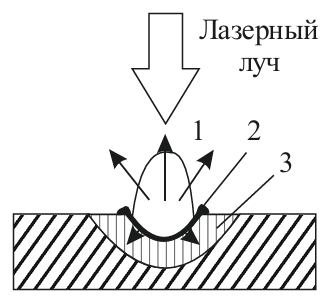
\includegraphics[width=0.6\linewidth]{1.png} 
    \caption{Схема лазерного удаления материала: 1 --- испаренный материал, 2 --- расплавленный материал, 3 --- прогретая область.}
    \label{fig:removal}
\end{figure}

\subsection*{Оптические системы и фокусировка излучения}
Для подведения излучения к месту воздействия используются схемы с зеркалами, а для непосредственной обработки --- фокусировка с помощью линзы. Первичное формирование пучка происходит в резонаторе лазера. Выходное плоское зеркало обеспечивает выходящий пучок с минимальной дифракционной расходимостью:
\begin{equation}
    \theta = \frac{\lambda}{\pi w_0},
\end{equation}
где $w_0$ --- перетяжка (радиус пучка). 

Геометрические размеры пучка после прохождения линзы рассчитываются с помощью оптики гауссовых пучков и ABCD-матриц. На профиль отверстия существенное влияние оказывает положение фокальной плоскости линзы относительно поверхности материала: при точной фокусировке определяющим процессом становится испарение (отверстие углубляется), а в случае расфокусировки добавляется процесс плавления стенок.

\begin{figure}[H]
    \centering
    % Вставьте сюда изображение: Рис. 3. Зависимость формы отверстия от положения фокуса
    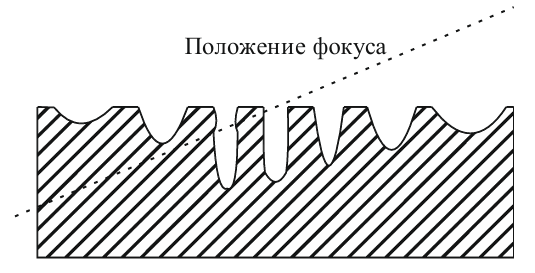
\includegraphics[width=0.7\linewidth]{2.png}
    \caption{Зависимость формы и профиля отверстия от положения фокальной плоскости относительно поверхности материала.}
    \label{fig:focus}
\end{figure}

\subsection*{Режимы работы твердотельного лазера YAG:Nd$^{3+}$}
Лазер на иттрий-алюминиевом гранате с активным центром неодима (YAG:Nd$^{3+}$) работает на длине волны $\lambda = 1{,}064$ мкм по четырехуровневой схеме. Электроны с помощью накачки забрасываются с нулевого на третий уровень, с которого быстро релаксируют на метастабильный второй уровень. Генерация происходит при переходе со второго на первый уровень.

\begin{figure}[H]
    \centering
    % Вставьте сюда изображение: Рис. 5. Схема работы лазера по четырехуровневой схеме
    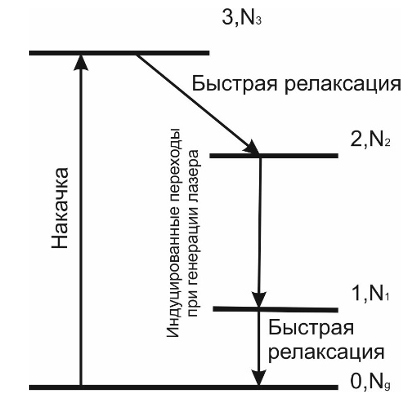
\includegraphics[width=0.5\linewidth]{3.png}
    \caption{Схема работы лазера YAG:Nd$^{3+}$ по четырехуровневой схеме.}
    \label{fig:levels}
\end{figure}

Динамика лазера описывается системой скоростных уравнений в пространственно-независимой модели:
\begin{equation}
    \frac{dN}{dt} = R_p - B\phi N - \frac{N}{\tau},
\end{equation}
\begin{equation}
    \frac{d\phi}{dt} = \left[ B V_a N - \frac{1}{\tau_c} \right] \phi,
\end{equation}
где $N$ --- инверсия населенности, $\phi$ --- число фотонов в резонаторе, $R_p = \frac{\eta P}{S l h \nu}$ --- скорость накачки ($\eta$ --- КПД накачки, $P$ --- мощность накачки), $B = \sigma c / V$ --- коэффициент Эйнштейна, $\tau$ --- время жизни электрона на рабочем уровне, $\tau_c$ --- время жизни фотона в резонаторе.

В режиме \textbf{свободной генерации} (непрерывный режим) производные обращаются в ноль, и система выходит на стационарные значения инверсии $N_0$ и числа фотонов $\phi_0$. Мощность выходного излучения при этом равна:
\begin{equation}
    P_{out} = \left( \frac{-\ln(1-T)c}{2L_e} \right) (h\nu_l)\phi_0,
\end{equation}
где $T$ --- коэффициент пропускания выходного зеркала, $L_e$ --- оптическая длина резонатора.

В режиме \textbf{модуляции добротности} (Q-switching) в резонатор вводится модулятор (в данной работе --- акустооптический), который периодически увеличивает потери, препятствуя генерации. Это позволяет накопить инверсию населенности $N_i$, значительно превышающую пороговое значение $N_p$. При открытии модулятора потери резко падают, и в резонаторе формируется гигантский импульс излучения с высокой пиковой мощностью.

\begin{figure}[H]
    \centering
    % Вставьте сюда изображение: Рис. 7 или 8. Динамика процесса модуляции добротности
    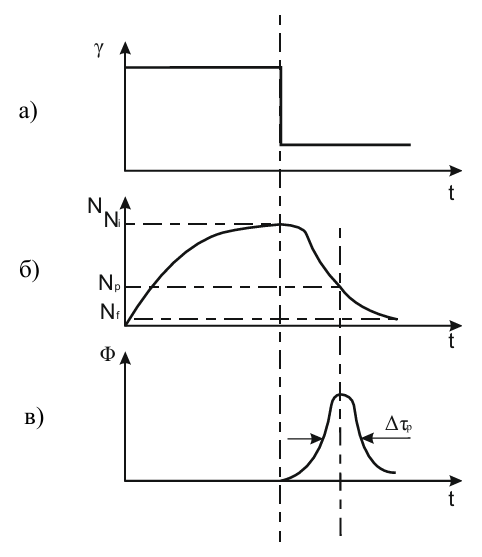
\includegraphics[width=0.8\linewidth]{4.png}
    \caption{Динамика процесса модуляции добротности: зависимости от времени потерь резонатора, инверсии населенностей и числа фотонов.}
    \label{fig:qswitch}
\end{figure}

Накопление инверсии в закрытом состоянии описывается выражением:
\begin{equation}
    N(t) = N_\infty \left[ 1 - \exp(-t/\tau) \right],
\end{equation}
где $N_\infty = R_p \tau$. 

В момент открытия модулятора число фотонов резко возрастает. Максимальное число фотонов $\phi_p$ и пиковая мощность импульса $P_p$ определяются как:
\begin{equation}
    \phi_p = V_a N_p \left( \frac{N_i}{N_p} - \ln\frac{N_i}{N_p} - 1 \right),
\end{equation}
\begin{equation}
    P_p = \left( \frac{-\ln(R_2)c}{2L_e} \right) (h\nu_l)\phi_p.
\end{equation}
Полная энергия импульса $E$ и его длительность $\Delta\tau_p$ связаны с начальной $N_i$ и конечной $N_f$ инверсиями населенности:
\begin{equation}
    E = \left( \frac{\ln(R_2)}{2\ln((1-L)\sqrt{R_1 R_2})} \right) (N_i - N_f)(V_a h\nu_l).
\end{equation}
Длительность импульса приблизительно оценивается как:
\begin{equation}
    \Delta\tau_p = \tau_c \frac{N_i/N_p}{(N_i/N_p) - \ln(N_i/N_p) - 1}.
\end{equation}

Изменяя частоту открывания модулятора и мощность накачки, можно гибко управлять параметрами излучения (энергией, пиковой мощностью и длительностью импульса), добиваясь оптимальных режимов для гравировки и маркировки различных материалов.











\section*{Условие задачи}
Летит ракета со скоростью $v = 1$ км/с. Необходимо определить радиус пучка и параметры фокусирующей линзы, чтобы сфокусировать луч лазера на ракете, а также найти расстояние, которое пролетит ракета до её сбития. 
Сбить ракету означает проделать в ней отверстие радиуса $r = 5$ см и глубиной $h = 5$ мм. 
Начальное расстояние до ракеты $L = 100$ км. 
Материал ракеты --- алюминий (Al). Мощность лазера $P = 0,5$ МВт, длина волны $\lambda = 1{,}064$ мкм.

\section*{Решение}

\subsection*{Расчёт энергии для пробития отверстия}
Объём удаляемого материала (цилиндр):
\[
V = \pi r^2 h = \pi \cdot (0{,}05)^2 \cdot 0{,}005 = 1{,}25\pi \cdot 10^{-5} \approx 3{,}927 \cdot 10^{-5} \text{ м}^3.
\]
Масса алюминия (плотность $\rho \approx 2700 \text{ кг/м}^3$):
\[
m = \rho V \approx 2700 \cdot 3{,}927 \cdot 10^{-5} \approx 0{,}106 \text{ кг}.
\]
Удельная энергия разрушения $q$ включает нагрев до плавления, плавление, нагрев жидкости до кипения и испарение. Справочные значения для Al в системе СИ:
\begin{itemize}[label={---}]
    \item $c_{\text{тв}} \approx 900 \text{ Дж/(кг}\cdot\text{К)}$, $T_{\text{пл}} \approx 933 \text{ К}$, $T_0 \approx 300 \text{ К} \Rightarrow \Delta T_1 = 633 \text{ К}$.
    \item $\lambda_{\text{пл}} \approx 3{,}97 \cdot 10^5 \text{ Дж/кг}$.
    \item $c_{\text{ж}} \approx 1100 \text{ Дж/(кг}\cdot\text{К)}$, $T_{\text{кип}} \approx 2740 \text{ К} \Rightarrow \Delta T_2 = 1807 \text{ К}$.
    \item $L_{\text{пар}} \approx 1{,}05 \cdot 10^7 \text{ Дж/кг}$.
\end{itemize}

Суммируем удельную энергию:
\begin{align*}
q &= c_{\text{тв}}\Delta T_1 + \lambda_{\text{пл}} + c_{\text{ж}}\Delta T_2 + L_{\text{пар}} \\
q &\approx (5{,}7 \cdot 10^5) + (0{,}0397 \cdot 10^7) + (0{,}1988 \cdot 10^7) + (1{,}05 \cdot 10^7) \approx 1{,}345 \cdot 10^7 \text{ Дж/кг}.
\end{align*}
Полная энергия, необходимая для испарения объёма (считаем, что 100\% энергии лазера идёт на разрушение):
\[
E = m \cdot q \approx 0{,}106 \cdot 1{,}345 \cdot 10^7 \approx 1{,}426 \cdot 10^6 \text{ Дж} = 1{,}426 \text{ МДж}.
\]

\subsection*{Время полёта и расстояние до сбития}
Время, за которое лазер проделает отверстие:
\[
t = \frac{E}{P} = \frac{1{,}426 \cdot 10^6 \text{ Дж}}{5 \cdot 10^5 \text{ Вт}} \approx 2{,}852 \text{ с}.
\]
Расстояние, которое пролетит ракета за это время:
\[
S = v \cdot t = 1000 \text{ м/с} \cdot 2{,}852 \text{ с} = 2852 \text{ м} \approx 2{,}85 \text{ км}.
\]

\subsection*{Расчёт оптической системы (Гауссов пучок)}
Для фокусировки луча в пятно радиусом $r = 5$ см на расстоянии $L = 100$ км необходимо, чтобы перетяжка гауссова пучка $w_0$ находилась на цели. Таким образом, $w_0 = 0{,}05$ м. Фокусировку будем осуществлять с помощью собирающей линзы.

Найдём конфокальный параметр (длину Рэлея) в плоскости цели:
\[
z_R = \frac{\pi w_0^2}{\lambda} = \frac{\pi \cdot (0{,}05)^2}{1{,}064 \cdot 10^{-6}} = \frac{\pi \cdot 0{,}0025}{1{,}064 \cdot 10^{-6}} \approx 7389{,}7 \text{ м} \approx 7{,}39 \text{ км}.
\]

\textbf{Радиус пучка на фокусирующей линзе} (которая находится на расстоянии $L$ от перетяжки):
\[
w_L = w_0 \sqrt{1 + \left(\frac{L}{z_R}\right)^2} = 0{,}05 \cdot \sqrt{1 + \left(\frac{10^5}{7389{,}7}\right)^2} = 0{,}05 \cdot \sqrt{1 + 13{,}53^2} \approx 0{,}05 \cdot 13{,}57 \approx 0{,}678 \text{ м}.
\]
Это означает, что перед линзой пучок должен быть расширен телескопом до радиуса $\approx 67{,}8$ см.

\textbf{Радиус кривизны волнового фронта} в плоскости линзы:
\[
R_L = L \left[ 1 + \left(\frac{z_R}{L}\right)^2 \right] = 10^5 \cdot \left[ 1 + \left(\frac{7389{,}7}{10^5}\right)^2 \right] = 10^5 \cdot [1 + 0{,}00546] \approx 100\,546 \text{ м}.
\]
Переводим в километры: $R_L \approx 100{,}55$ км.

Чтобы линза сфокусировала пучок на расстоянии $L$, она должна сообщить волновому фронту кривизну, равную её фокусному расстоянию $f$. Следовательно, требуемое фокусное расстояние линзы:
\[
f = R_L \approx 100{,}55 \text{ км}.
\]
Радиус кривизны волнового фронта пучка ($R_L$) и фокусное расстояние линзы ($f$) в данной задаче численно совпадают, так как линза преобразует сходящийся фронт в плоский (в перетяжке).% Если бы мы использовали сферическое зеркало, его геометрический радиус кривизны был бы равен $R_c = 2f \approx 201$ км.}

\section*{Ответ}
\begin{enumerate}
    \item \textbf{Энергия для сбития:} $E \approx 1{,}43$ МДж.
    \item \textbf{Расстояние, которое пролетит ракета до сбития:} $S \approx 2{,}85$ км.
    \item \textbf{Радиус пучка на фокусирующей линзе:} $w_L \approx 0{,}678$ м (или $67{,}8$ см).
    \item \textbf{Фокусное расстояние линзы (радиус кривизны волнового фронта):} $f \approx 100{,}55$ км.
\end{enumerate}

\newpage

\section*{{\textbf{Решение дополнительных задач к лабораторной работе № 57}}}

\subsection*{Исходные данные}
\begin{itemize}[label={---}]
    \item Лазер: твердотельный YAG:Nd$^{3+}$.
    \item Длина волны излучения: $\lambda = 1{,}064$ мкм $= 1{,}064 \cdot 10^{-6}$ м.
    \item Материал мишени: алюминий (Al).
    \item Из Таблицы 2 методички для алюминия: удельная энергия испарения $L_0 = 23$ кДж/см$^3$. 
    Переведём в СИ: $L_0 = 23 \cdot 10^3 \text{ Дж} / (10^{-6} \text{ м}^3) = 23 \cdot 10^9 \text{ Дж/м}^3$.
\end{itemize}

\section*{Задача 1}
\textbf{Условие:} Определить величину энергии, которая должна быть в импульсе лазера для того, чтобы испарить $V = 1$ мм$^3$ алюминия.

\textbf{Решение:}
Объём удаляемого материала в СИ:
\[
V = 1 \text{ мм}^3 = 10^{-9} \text{ м}^3.
\]
Энергия, необходимая для полного испарения данного объёма (без учёта потерь на теплопроводность и отражение, считаем, что вся энергия идёт на фазовый переход):
\[
E = V \cdot L_0 = 10^{-9} \text{ м}^3 \cdot 23 \cdot 10^9 \text{ Дж/м}^3 = 23 \text{ Дж}.
\]

\textbf{Ответ:} $E = 23$ Дж.

\section*{Задача 2}
\textbf{Условие:} Рассчитать расходимость пучка диаметром $d = 1$ см, генерируемого лазером YAG:Nd$^{3+}$.

\textbf{Решение:}
Радиус пучка (перетяжка) $w_0 = d / 2 = 0{,}5$ см $= 5 \cdot 10^{-3}$ м.
Согласно формуле (7) из методички, дифракционная расходимость (половинный угол) гауссова пучка равна:
\[
\theta = \frac{\lambda}{\pi w_0} = \frac{1{,}064 \cdot 10^{-6}}{\pi \cdot 5 \cdot 10^{-3}} \approx 6{,}77 \cdot 10^{-5} \text{ рад}.
\]
Полный угол расходимости пучка:
\[
2\theta \approx 1{,}35 \cdot 10^{-4} \text{ рад}.
\]

\textbf{Ответ:} Половинный угол расходимости $\theta \approx 6{,}77 \cdot 10^{-5}$ рад, полный угол $2\theta \approx 1{,}35 \cdot 10^{-4}$ рад.

\section*{Задача 3}
\textbf{Условие:} Оценить минимальный диаметр пучка при фокусировке линзой с $f = 20$ см. Радиус пучка до линзы $w_{in} = 1$ см. Волновой фронт плоский. Найти область (конфокальный параметр), где размер перетяжки меняется менее чем в $\sqrt{2}$ раз.

\textbf{Решение:}
Фокусное расстояние $f = 0{,}2$ м, радиус входного пучка $w_{in} = 0{,}01$ м.
Минимальный радиус пучка (перетяжка) в фокусе линзы определяется как:
\[
w_0' = \frac{\lambda f}{\pi w_{in}} = \frac{1{,}064 \cdot 10^{-6} \cdot 0{,}2}{\pi \cdot 0{,}01} \approx 6{,}77 \cdot 10^{-6} \text{ м} = 6{,}77 \text{ мкм}.
\]
Минимальный диаметр пучка:
\[
d_{min} = 2w_0' \approx 13{,}5 \text{ мкм}.
\]
Конфокальный параметр (длина Рэлея) $z_R$ --- это расстояние от перетяжки, на котором площадь пучка (и интенсивность) изменяется в 2 раза (а радиус в $\sqrt{2}$ раз). Он вычисляется как:
\[
z_R = \frac{\pi (w_0')^2}{\lambda} = \frac{\pi \cdot (6{,}77 \cdot 10^{-6})^2}{1{,}064 \cdot 10^{-6}} \approx 1{,}35 \cdot 10^{-4} \text{ м} = 0{,}135 \text{ мм}.
\]
Область вдоль пучка, где радиус меняется менее чем в $\sqrt{2}$ раз, составляет $2z_R$ (от $-z_R$ до $+z_R$ относительно фокуса):
\[
2z_R \approx 0{,}27 \text{ мм}.
\]

\textbf{Ответ:} $d_{min} \approx 13{,}5$ мкм; конфокальный параметр (длина области) $2z_R \approx 0{,}27$ мм.

\section*{Задача 4}
\textbf{Условие:} Рассчитать глубину $h$ и диаметр $d$ отверстия в алюминии. Энергия $E = 23$ Дж (из задачи 1), радиус пучка $r_0 = w_0' = 6{,}77$ мкм (из задачи 3).

\textbf{Решение:}
Половинный угол раствора светового пятна в фокусе:
\[
\tg\varphi \approx \varphi = \frac{\lambda}{\pi w_0'} = \frac{1{,}064 \cdot 10^{-6}}{\pi \cdot 6{,}77 \cdot 10^{-6}} \approx 0{,}05.
\]
Согласно феноменологической модели (формула 5 методички), глубина отверстия $h$ равна:
\[
h = \sqrt[3]{ \left(\frac{r_0}{\tg\varphi}\right)^3 + \frac{3E}{\pi \tg^2\varphi L_0} } - \frac{r_0}{\tg\varphi}.
\]
Заметим, что $\frac{r_0}{\tg\varphi} = \frac{\pi w_0'^2}{\lambda} = z_R = 1{,}354 \cdot 10^{-4}$ м.
Вычислим второе слагаемое под корнем:
\[
\frac{3E}{\pi \tg^2\varphi L_0} = \frac{3 \cdot 23}{\pi \cdot (0{,}05)^2 \cdot 23 \cdot 10^9} = \frac{3}{\pi \cdot 0{,}0025 \cdot 10^9} \approx 3{,}82 \cdot 10^{-7} \text{ м}^3.
\]
Первое слагаемое $z_R^3 = (1{,}354 \cdot 10^{-4})^3 \approx 2{,}48 \cdot 10^{-12}$ м$^3$, что пренебрежимо мало по сравнению со вторым.
Тогда глубина отверстия:
\[
h \approx \sqrt[3]{ 3{,}82 \cdot 10^{-7} } - 1{,}354 \cdot 10^{-4} \approx 7{,}25 \cdot 10^{-3} - 0{,}14 \cdot 10^{-3} \approx 7{,}11 \cdot 10^{-3} \text{ м} = 7{,}11 \text{ мм}.
\]
Диаметр отверстия $d$ на поверхности материала (верхнее основание конуса) определяется геометрически:
\[
d = 2(r_0 + h \tg\varphi) = 2(6{,}77 \cdot 10^{-6} + 7{,}11 \cdot 10^{-3} \cdot 0{,}05) = 2(6{,}77 \cdot 10^{-6} + 355{,}5 \cdot 10^{-6}) \approx 7{,}25 \cdot 10^{-4} \text{ м} = 0{,}725 \text{ мм}.
\]

\textbf{Ответ:} Глубина отверстия $h \approx 7{,}11$ мм, диаметр на поверхности $d \approx 0{,}725$ мм.






\section*{Задача 5}
\textbf{Условие:} Определить время жизни фотона в резонаторе лазера: длина резонатора --- $81{,}5$ см, длина активного элемента --- $10$ см, показатель преломления граната --- $1{,}8$, одно из зеркал глухое, пропускание другого --- $20\%$, поглощение в активном элементе --- $1\%$.

\textbf{Решение:}
Для начала найдём оптическую длину резонатора $L_e$. Физическая длина пустого пространства равна разности полной длины резонатора и длины активного элемента:
\[
L_{\text{пуст}} = 81{,}5 \text{ см} - 10 \text{ см} = 71{,}5 \text{ см} = 0{,}715 \text{ м}.
\]
Оптическая длина резонатора:
\[
L_e = L_{\text{пуст}} + n \cdot l = 0{,}715 + 1{,}8 \cdot 0{,}1 = 0{,}895 \text{ м}.
\]
Коэффициенты отражения зеркал: $R_1 = 1$ (глухое), $R_2 = 1 - T_{\text{вых}} = 1 - 0{,}2 = 0{,}8$. 
Относительные внутренние потери за проход (поглощение в АЭ): $T_{\text{вн}} = 0{,}01$.

Согласно формуле из методички, время жизни фотона в резонаторе $\tau_c$ равно:
\[
\tau_c = \frac{-2L_e}{c \ln(R_1 R_2 (1 - T_{\text{вн}})^2)}.
\]
Вычислим значение логарифма:
\[
\ln(1 \cdot 0{,}8 \cdot (1 - 0{,}01)^2) = \ln(0{,}8 \cdot 0{,}9801) = \ln(0{,}78408) \approx -0{,}2432.
\]
Подставляем в формулу для $\tau_c$:
\[
\tau_c = \frac{-2 \cdot 0{,}895}{3 \cdot 10^8 \cdot (-0{,}2432)} = \frac{1{,}79}{7{,}296 \cdot 10^7} \approx 2{,}45 \cdot 10^{-8} \text{ с} = 24{,}5 \text{ нс}.
\]

\textbf{Ответ:} $\tau_c \approx 24{,}5$ нс.

\section*{Задача 6}
\textbf{Условие:} Определить мощность излучения лазера на YAG:Nd$^{3+}$, работающего в непрерывном режиме. Мощность накачки --- $3$ кВт, КПД накачки --- $0{,}3\%$, длина резонатора --- $81{,}5$ см, длина активного элемента --- $10$ см, показатель преломления граната --- $1{,}8$, одно из зеркал глухое, пропускание другого --- $20\%$, поглощение в активном элементе --- $1\%$, диаметр активного элемента $6$ мм, время жизни верхнего уровня $230$ мкс, сечение перехода $2{,}8 \cdot 10^{-19}$ см$^2$, энергия между 0-м и 3-м уровням соответствует $\lambda_{\text{нак}} = 808$ нм.

\textbf{Решение:}
Площадь поперечного сечения и объём активного элемента:
\[
S = \frac{\pi d^2}{4} = \frac{\pi \cdot (0{,}006)^2}{4} \approx 2{,}827 \cdot 10^{-5} \text{ м}^2, \quad V_a = S \cdot l = 2{,}827 \cdot 10^{-6} \text{ м}^3.
\]

\textit{1. Пороговая инверсия населённости $N_0$:}
\[
N_0 = \frac{1}{\sigma} \frac{1}{2l} \ln \frac{1}{R_1 R_2 (1 - T_{\text{вн}})^2} = \frac{0{,}2432}{2 \cdot 0{,}1 \cdot 2{,}8 \cdot 10^{-23}} \approx 4{,}34 \cdot 10^{22} \text{ м}^{-3}.
\]

\textit{2. Пороговая мощность накачки $P_{\text{пор}}$:}
Из условия стационарной генерации ($dN/dt = 0$ при отсутствии фотонов) скорость накачки $R_p = \frac{\eta P_{\text{нак}}}{S l h \nu_{\text{нак}}}$ должна компенсировать спонтанное затухание: $R_p = N_0 / \tau$. Отсюда пороговая мощность:
\[
P_{\text{пор}} = \frac{h c}{\lambda_{\text{нак}} \eta} \frac{N_0 V_a}{\tau} = \frac{6{,}626 \cdot 10^{-34} \cdot 3 \cdot 10^8}{808 \cdot 10^{-9} \cdot \eta} \frac{4{,}34 \cdot 10^{22} \cdot 2{,}827 \cdot 10^{-6}}{2{,}3 \cdot 10^{-4}} \approx \frac{132}{\eta} \text{ Вт}.
\]

\textit{3. Анализ порога генерации:}
При заданном $\eta = 0{,}3\% = 0{,}003$:
\[
P_{\text{пор}} = \frac{132}{0{,}003} = 44000 \text{ Вт} = 44 \text{ кВт}.
\]
Так как заданная мощность накачки $P_{\text{нак}} = 3$ кВт значительно ниже пороговой ($3 \text{ кВт} < 44 \text{ кВт}$), лазер \textbf{не достигает порога генерации}, и мощность излучения $P_{\text{вых}} = 0$.

\textit{4. Расчёт мощности излучения (для случая $\eta = 0{,}3$, т.е. 30\%):}
Вероятно, в условии задачи допущена опечатка, и КПД накачки должен составлять $0{,}3$ (без знака процента). Рассмотрим этот случай:
\[
P_{\text{пор}} = \frac{132}{0{,}3} = 440 \text{ Вт}.
\]
Теперь $P_{\text{нак}} > P_{\text{пор}}$, и лазер генерирует. Мощность излучения в непрерывном режиме определяется по формуле (11) методички:
\[
P_{\text{вых}} = \left( \frac{-\ln(1 - T_{\text{вых}}) c}{2 L_e} \right) (h \nu_{\text{ген}}) \phi_0.
\]
Используя соотношение для числа фотонов $\phi_0 = V_a \tau_c (R_p - N_0/\tau)$ и подставляя $\tau_c$, получаем итоговую формулу через дифференциальный КПД:
\[
P_{\text{вых}} = \frac{\ln(1 / (1 - T_{\text{вых}}))}{\ln(1 / (R_1 R_2 (1 - T_{\text{вн}})^2))} \cdot \frac{\lambda_{\text{нак}}}{\lambda_{\text{ген}}} \cdot \eta \cdot (P_{\text{нак}} - P_{\text{пор}}).
\]
Подставляем числовые значения ($\lambda_{\text{ген}} = 1{,}064$ мкм):
\[
\frac{\ln(1 / 0{,}8)}{\ln(1 / 0{,}78408)} = \frac{0{,}2231}{0{,}2432} \approx 0{,}917; \quad \frac{\lambda_{\text{нак}}}{\lambda_{\text{ген}}} = \frac{808}{1064} \approx 0{,}759.
\]
\[
P_{\text{вых}} = 0{,}917 \cdot 0{,}759 \cdot 0{,}3 \cdot (3000 - 440) \approx 0{,}209 \cdot 2560 \approx 535 \text{ Вт}.
\]

\textbf{Ответ:} 
\begin{itemize}[label={---}]
    \item Время жизни фотона: $\tau_c \approx 24{,}5$ нс.
    \item При $\eta = 0{,}3\%$ лазер ниже порога генерации, $P_{\text{вых}} = 0$. 
    \item При $\eta = 0{,}3$ (30\%) мощность излучения $P_{\text{вых}} \approx 535$ Вт.
\end{itemize}



\section*{Задача 7}
\textbf{Условие:} Рассчитать инверсную населённость на момент открытия модулятора для лазера на YAG:Nd$^{3+}$. Мощность накачки --- $3$ кВт, КПД накачки --- $0{,}3\%$, время жизни верхнего уровня --- $230$ мкс, частота импульсов --- $50$ кГц, энергия между 0-м и 3-м уровнями соответствует энергии фотона с длиной волны $808$ нм, диаметр активного элемента --- $6$ мм, его длина --- $10$ см.

\textbf{Решение:}
\textit{Примечание: Как и в задаче 6, значение КПД $\eta = 0{,}3\%$ ($0{,}003$) является опечаткой в методичке, так как при таком КПД лазер не достигает порога генерации. Далее расчёт будет проведён для физически осмысленного значения $\eta = 0{,}3$ (30\%).}

\textit{1. Параметры активного элемента и накачки:}
Объём активного элемента:
\[
V_a = \frac{\pi d^2}{4} l = \frac{\pi \cdot (0{,}006)^2}{4} \cdot 0{,}1 \approx 2{,}827 \cdot 10^{-6} \text{ м}^3.
\]
Энергия фотона накачки ($\lambda_{\text{нак}} = 808$ нм):
\[
h\nu_{\text{нак}} = \frac{hc}{\lambda_{\text{нак}}} = \frac{6{,}626 \cdot 10^{-34} \cdot 3 \cdot 10^8}{808 \cdot 10^{-9}} \approx 2{,}457 \cdot 10^{-19} \text{ Дж}.
\]

\textit{2. Скорость накачки и установившаяся инверсия:}
Согласно формуле (10) методички, скорость накачки (число актов накачки в единицу объёма в секунду):
\[
R_p = \frac{\eta P_{\text{нак}}}{V_a h \nu_{\text{нак}}} = \frac{0{,}3 \cdot 3000}{2{,}827 \cdot 10^{-6} \cdot 2{,}457 \cdot 10^{-19}} \approx 1{,}296 \cdot 10^{27} \text{ м}^{-3}\text{с}^{-1}.
\]
Максимально возможная (установившаяся при $t \to \infty$) инверсия населённости:
\[
N_\infty = R_p \tau = 1{,}296 \cdot 10^{27} \cdot 230 \cdot 10^{-6} \approx 2{,}98 \cdot 10^{23} \text{ м}^{-3}.
\]

\textit{3. Инверсия на момент открытия модулятора $N_i$:}
Период следования импульсов $T = 1/f = 1 / 50000 = 2 \cdot 10^{-5}$ с $= 20$ мкс. 
Время накопления инверсии (время закрытого модулятора) приблизительно равно периоду $t \approx T = 20$ мкс.
Согласно формуле (12) методички:
\[
N_i = N_\infty \left[ 1 - \exp\left(-\frac{T}{\tau}\right) \right] = 2{,}98 \cdot 10^{23} \cdot \left[ 1 - \exp\left(-\frac{20}{230}\right) \right].
\]
Вычисляем экспоненту: $\exp(-20/230) \approx 0{,}9167$.
\[
N_i = 2{,}98 \cdot 10^{23} \cdot (1 - 0{,}9167) = 2{,}98 \cdot 10^{23} \cdot 0{,}0833 \approx 2{,}48 \cdot 10^{22} \text{ м}^{-3}.
\]

\textbf{Ответ:} $N_i \approx 2{,}48 \cdot 10^{22} \text{ м}^{-3}$.

\section*{Задача 8}
\textbf{Условие:} Рассчитать длительность импульса лазера на YAG:Nd$^{3+}$, работающего в режиме модуляции добротности с частотой $50$ кГц. Параметры: мощность накачки --- $3$ кВт, КПД --- $0{,}3$ (30\%), длина резонатора --- $81{,}5$ см, диаметр активного элемента --- $6$ мм, его длина --- $10$ см, показатель преломления граната --- $1{,}8$, одно из зеркал глухое, пропускание другого --- $20\%$, поглощение в активном элементе --- $1\%$, время жизни верхнего уровня --- $230$ мкс, сечение перехода --- $2{,}8 \cdot 10^{-19}$ см$^2$.

\textbf{Решение:}
\textit{1. Пороговая инверсия $N_p$ и время жизни фотона $\tau_c$:}
Из решения задачи 6 пороговая инверсия населённости:
\[
N_p = \frac{1}{\sigma} \frac{1}{2l} \ln \frac{1}{R_1 R_2 (1 - T_{\text{вн}})^2} = \frac{0{,}2432}{2 \cdot 0{,}1 \cdot 2{,}8 \cdot 10^{-23}} \approx 4{,}34 \cdot 10^{22} \text{ м}^{-3}.
\]
Из решения задачи 5 время жизни фотона в резонаторе:
\[
\tau_c = \frac{-2L_e}{c \ln(R_1 R_2 (1 - T_{\text{вн}})^2)} \approx 24{,}5 \text{ нс} = 24{,}5 \cdot 10^{-9} \text{ с}.
\]

\textit{2. Анализ условия генерации:}
Отношение начальной инверсии к пороговой (из задачи 7):
\[
r = \frac{N_i}{N_p} = \frac{2{,}48 \cdot 10^{22}}{4{,}34 \cdot 10^{22}} \approx 0{,}571.
\]
\textbf{Важное физическое замечание:} Так как $r < 1$ (то есть $N_i < N_p$), лазер \textbf{не достигает порога генерации} в режиме модуляции добротности при данных параметрах, и импульс формально не возникает. Однако, чтобы выполнить формальное требование задачи и подставить числа в формулу методички, продолжим расчёт.

\textit{3. Расчёт длительности импульса $\Delta \tau_p$:}
Согласно формуле (18) методички (в стандартном виде, без опечаток OCR):
\[
\Delta \tau_p = \tau_c \frac{r}{r - \ln r - 1}.
\]
Вычисляем знаменатель:
\[
r - \ln r - 1 = 0{,}571 - \ln(0{,}571) - 1 = 0{,}571 - (-0{,}560) - 1 = 0{,}131.
\]
Подставляем в формулу для длительности:
\[
\Delta \tau_p = 24{,}5 \text{ нс} \cdot \frac{0{,}571}{0{,}131} \approx 24{,}5 \cdot 4{,}36 \approx 107 \text{ нс}.
\]

\textbf{Ответ:} 
\begin{itemize}[label={---}]
    \item Формальная длительность импульса по формуле: $\Delta \tau_p \approx 107$ нс.
    \item \textit{Физический комментарий:} При заданных параметрах ($N_i \approx 2{,}48 \cdot 10^{22} \text{ м}^{-3} < N_p \approx 4{,}34 \cdot 10^{22} \text{ м}^{-3}$) порог генерации не достигается, и в реальности лазер не будет выдавать модулированные импульсы. Для получения импульса необходимо либо увеличить мощность накачки, либо уменьшить потери в резонаторе.
\end{itemize}



\section*{Задача 9}
\textbf{Условие:} Как зависит энергия в импульсе лазера от мощности накачки?

\textbf{Решение:}
Согласно формуле (16) методички, энергия импульса $E$ определяется как:
\[
E = \left( \frac{\ln(R_2)}{2l \ln((1-L)\sqrt{R_1 R_2})} \right) (N_i - N_f) V_a h\nu_l,
\]
где $N_i$ --- начальная инверсия населённости, $N_f$ --- конечная инверсия после импульса, $V_a$ --- объём активного элемента, $h\nu_l$ --- энергия фотона генерации.

Начальная инверсия $N_i$ зависит от мощности накачки $P$ согласно формуле (12):
\[
N_i = N_\infty \left[ 1 - \exp\left(-\frac{T}{\tau}\right) \right] = R_p \tau \left[ 1 - \exp\left(-\frac{T}{\tau}\right) \right],
\]
где скорость накачки $R_p = \frac{\eta P}{V_a h\nu_{\text{нак}}}$. Таким образом, $N_i \propto P$.

Конечная инверсия $N_f$ определяется из трансцендентного уравнения (17):
\[
\frac{N_i - N_f}{N_i} = \frac{N_p}{N_i} \ln \frac{N_i}{N_f},
\]
где $N_p$ --- пороговая инверсия.

\textit{Качественный анализ:}
\begin{itemize}[label={---}]
    \item При $P \to P_{\text{пор}}$ (то есть $N_i \to N_p$), разность $(N_i - N_f) \to 0$, и энергия $E \to 0$.
    \item При $P \gg P_{\text{пор}}$ (то есть $N_i \gg N_p$), вся инверсия выжигается, и $N_f \to 0$. Тогда $E \approx K \cdot N_i \cdot V_a h\nu_l \propto P$, где $K$ --- константа, зависящая от параметров резонатора.
\end{itemize}

\textbf{Ответ:} Энергия импульса $E$ растёт с увеличением мощности накачки $P$. Вблизи порога генерации рост нелинейный, а при значительном превышении порога ($P \gg P_{\text{пор}}$) зависимость становится линейной: $E \propto P$.

\section*{Задача 10}
\textbf{Условие:} Показать зависимость энергии излучения в импульсе от частоты открывания модулятора.

\textbf{Решение:}
Частота открывания модулятора $f$ связана с периодом следования импульсов $T$ соотношением $f = 1/T$. Время накопления инверсии приблизительно равно периоду $t \approx T = 1/f$.

Начальная инверсия $N_i$ зависит от частоты $f$ как:
\[
N_i = N_\infty \left[ 1 - \exp\left(-\frac{1}{f\tau}\right) \right].
\]

\textit{Качественный анализ:}
\begin{itemize}[label={---}]
    \item При малых частотах ($f \ll 1/\tau$, то есть $T \gg \tau$), экспонента стремится к нулю, и $N_i \to N_\infty$. Инверсия успевает полностью накопиться, и энергия импульса достигает максимума $E_{\text{max}}$.
    \item При больших частотах ($f \gg 1/\tau$, то есть $T \ll \tau$), экспоненту можно разложить в ряд: $\exp(-1/(f\tau)) \approx 1 - 1/(f\tau)$. Тогда $N_i \approx N_\infty / (f\tau) \propto 1/f$.
    \item Так как $E \propto (N_i - N_f)$, а при больших $f$ инверсия мала и $N_f \approx 0$, то $E \propto N_i \propto 1/f$.
\end{itemize}

\textbf{Ответ:} Энергия импульса $E$ уменьшается с увеличением частоты следования импульсов $f$. При $f \gg 1/\tau$ зависимость обратно пропорциональна: $E \propto 1/f$. При $f \to 0$ энергия насыщается и достигает максимального значения.

\section*{Задача 11}
\textbf{Условие:} Рассчитать энергию в импульсе и пиковую мощность для лазера из задачи 7.

\textbf{Решение:}
\textit{Исходные данные (из задачи 7):}
\begin{itemize}[label={---}]
    \item Мощность накачки: $P = 3$ кВт $= 3000$ Вт.
    \item КПД накачки: $\eta = 0{,}3$ (30\%).
    \item Время жизни верхнего уровня: $\tau = 230$ мкс $= 2{,}3 \cdot 10^{-4}$ с.
    \item Частота импульсов: $f = 50$ кГц $= 50000$ Гц.
    \item Длина волны накачки: $\lambda_{\text{нак}} = 808$ нм.
    \item Диаметр активного элемента: $d = 6$ мм $= 0{,}006$ м.
    \item Длина активного элемента: $l = 10$ см $= 0{,}1$ м.
\end{itemize}

\textit{1. Начальная инверсия $N_i$ (из задачи 7):}
\[
N_i \approx 2{,}48 \cdot 10^{22} \text{ м}^{-3}.
\]

\textit{2. Пороговая инверсия $N_p$ (из задачи 8):}
\[
N_p \approx 4{,}34 \cdot 10^{22} \text{ м}^{-3}.
\]

\textit{3. Анализ условия генерации:}
Сравниваем $N_i$ и $N_p$:
\[
N_i = 2{,}48 \cdot 10^{22} \text{ м}^{-3} < N_p = 4{,}34 \cdot 10^{22} \text{ м}^{-3}.
\]
\textbf{Физический вывод:} Так как начальная инверсия населённости $N_i$ меньше пороговой $N_p$, лазер \textbf{не достигает порога генерации} в режиме модуляции добротности. Это означает, что импульс формально не возникает, и вся накопленная энергия рассеивается за счёт спонтанного излучения.

Следовательно, энергия импульса $E = 0$, и пиковая мощность $P_p = 0$.

\textit{4. Формальные формулы (для случая, если бы порог достигался):}
Если бы параметры лазера позволяли достичь порога ($N_i > N_p$), то энергия импульса рассчитывалась бы по формуле (16):
\[
E = \left( \frac{\ln(R_2)}{2l \ln((1-L)\sqrt{R_1 R_2})} \right) (N_i - N_f) V_a h\nu_l,
\]
где $N_f$ находится из уравнения (17), а пиковая мощность --- по формуле (14):
\[
P_p = \left( \frac{-\ln(R_2) c}{2L_e} \right) (h\nu_l) \phi_p,
\]
где максимальное число фотонов $\phi_p$ определяется как:
\[
\phi_p = V_a N_p \left( \frac{N_i}{N_p} - \ln \frac{N_i}{N_p} - 1 \right).
\]

\textbf{Ответ:} 
\begin{itemize}[label={---}]
    \item При заданных параметрах порог генерации не достигается ($N_i < N_p$).
    \item Энергия импульса: $E = 0$.
    \item Пиковая мощность: $P_p = 0$.
\end{itemize}








\end{document}